%!TeX encoding = UTF-8
%!TeX program = xelatex
\documentclass[
  notheorems,
  aspectratio=54,
]{beamer}

%% preamble
\title{An Introduction to Synchronization on Complex Networks}
% \subtitle{The subtitle}
\author{Jingsheng Gao}
\institute{Anqing Normal University}

\useoutertheme{shadow}
\setbeamertemplate{headline}{}
\mode<presentation>{
  \usetheme{Warsaw}
  \usecolortheme{seagull}
}

\setbeamertemplate{footline}
{
  \leavevmode%
  \hbox{%
  \begin{beamercolorbox}[wd=.45\paperwidth,ht=2.25ex,dp=1ex,center]{title in head/foot}%
    \usebeamerfont{title in head/foot}\inserttitle
  \end{beamercolorbox}%
  \begin{beamercolorbox}[wd=.45\paperwidth,ht=2.25ex,dp=1ex,center]{author in head/foot}%
      \usebeamerfont{author in head/foot}\insertauthor\ - \insertinstitute
  \end{beamercolorbox}%
  \begin{beamercolorbox}[wd=.1\paperwidth,ht=2.25ex,dp=1ex,right]{date in head/foot}%
    \insertframenumber{} / \inserttotalframenumber\hspace*{2ex} 
  \end{beamercolorbox}}%
  \vskip0pt%
}


\setbeamertemplate{navigation symbols}{}

\usepackage[
    backend=biber,
    autocite=superscript,
    sorting=none
]{biblatex}
\AtBeginBibliography{\small}
\addbibresource{refs.bib}

\usepackage{caption}
\captionsetup[figure]{font=scriptsize}

\usepackage{latexsym}
\usepackage{amsmath,amssymb}
\usepackage{mathtools}
\usepackage{color,xcolor}
\usepackage{graphicx}
\usepackage{algorithm}
\usepackage{amsthm}
\usepackage{lmodern}
% \usepackage[UTF8]{ctex}
% \usepackage{xeCJK}
\usepackage{animate} % insert gif

\usepackage{lipsum}
\usepackage{ulem}

\usepackage{listings} % display code on slides; don't forget [fragile] option after \begin{frame}

% ----------------------------------------------
% tikx
\usepackage{framed}
\usepackage{tikz}
\usepackage{pgf}
\usetikzlibrary{calc,trees,positioning,arrows,chains,shapes.geometric,%
    decorations.pathreplacing,decorations.pathmorphing,shapes,%
    matrix,shapes.symbols}



% ----------------------------------------------

% ---------------------------------------------------------------------
% Jet Black Theme
% \setbeamercolor{normal text}{fg=white,bg=black!90}
% \setbeamercolor{structure}{fg=white}
%
% \setbeamercolor{alerted text}{fg=red!85!black}
%
% \setbeamercolor{item projected}{use=item,fg=black,bg=item.fg!35}
%
% \setbeamercolor*{palette primary}{use=structure,fg=structure.fg}
% \setbeamercolor*{palette secondary}{use=structure,fg=structure.fg!95!black}
% \setbeamercolor*{palette tertiary}{use=structure,fg=structure.fg!90!black}
% \setbeamercolor*{palette quaternary}{use=structure,fg=structure.fg!95!black,bg=black!80}
%
% \setbeamercolor*{framesubtitle}{fg=white}
%
% \setbeamercolor*{block title}{parent=structure,bg=black!70!gray}
% \setbeamercolor*{block body}{fg=black,bg=black!10}
% \setbeamercolor*{block title alerted}{parent=alerted text,bg=black!15}
% \setbeamercolor*{block title example}{parent=example text,bg=black!15}
% ---------------------------------------------------------------------


% \newcommand{\reditem}[1]{\setbeamercolor{item}{fg=red}\item #1}

% \newcommand*{\Scale}[2][4]{\scalebox{#1}{\ensuremath{#2}}}

% -------------------------------------------------------------

% -------------------------------------------------------------

\begin{document}

% title frame
\begin{frame}
    \titlepage
\end{frame}

\begin{frame}{Introduction}
 \begin{itemize}
    \item Synchronization on complex networks is a fascinating phenomenon that explores how interconnected systems can achieve coordinated behavior.
    \item Among collective phenomena in natural and social systems, the synchronization of a set of interacting individuals or units has been intensively studied because of its ubiquity in the natural world.
    \item It is applied on engineering systems, biological systems, social dynamics, and more
  \end{itemize}
\end{frame}

\begin{frame}{1. Synchronization}
  \begin{figure}
    \centering
  \end{figure}
  \begin{itemize}
    \item Synchronization is the process by which components of a system adjust their behavior to a common rhythm or pattern.
    \item Metronome synchronization, firefly flashing, circadian rhythms, brain networks.
\begin{figure}
  \begin{minipage}[b]{0.45\textwidth}
    \textbf{Schooling Fish}\par\medskip
    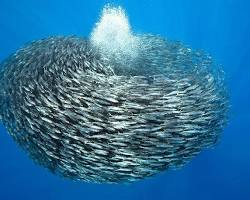
\includegraphics[width=0.4\textwidth]{schooling_fish.png}
  \end{minipage}
  \hfill
  \begin{minipage}[b]{0.45\textwidth}
    \textbf{Bioluminescence in Oceans}\par\medskip
    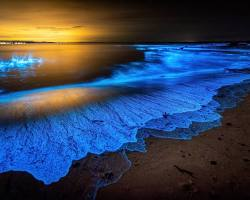
\includegraphics[width=0.4\textwidth]{bioluminescence.png}
  \end{minipage}
\end{figure}
  \end{itemize}
\end{frame}

\begin{frame}{3.1 Scale-free network}
  \begin{itemize}
   \item A scale-free network\cite{wiki:scale_free_network} is a network whose degree distribution follows a power law, at least asymptotically.
  \end{itemize}
  \begin{figure}
    \centering
    \textbf{Examples}\par\medskip
    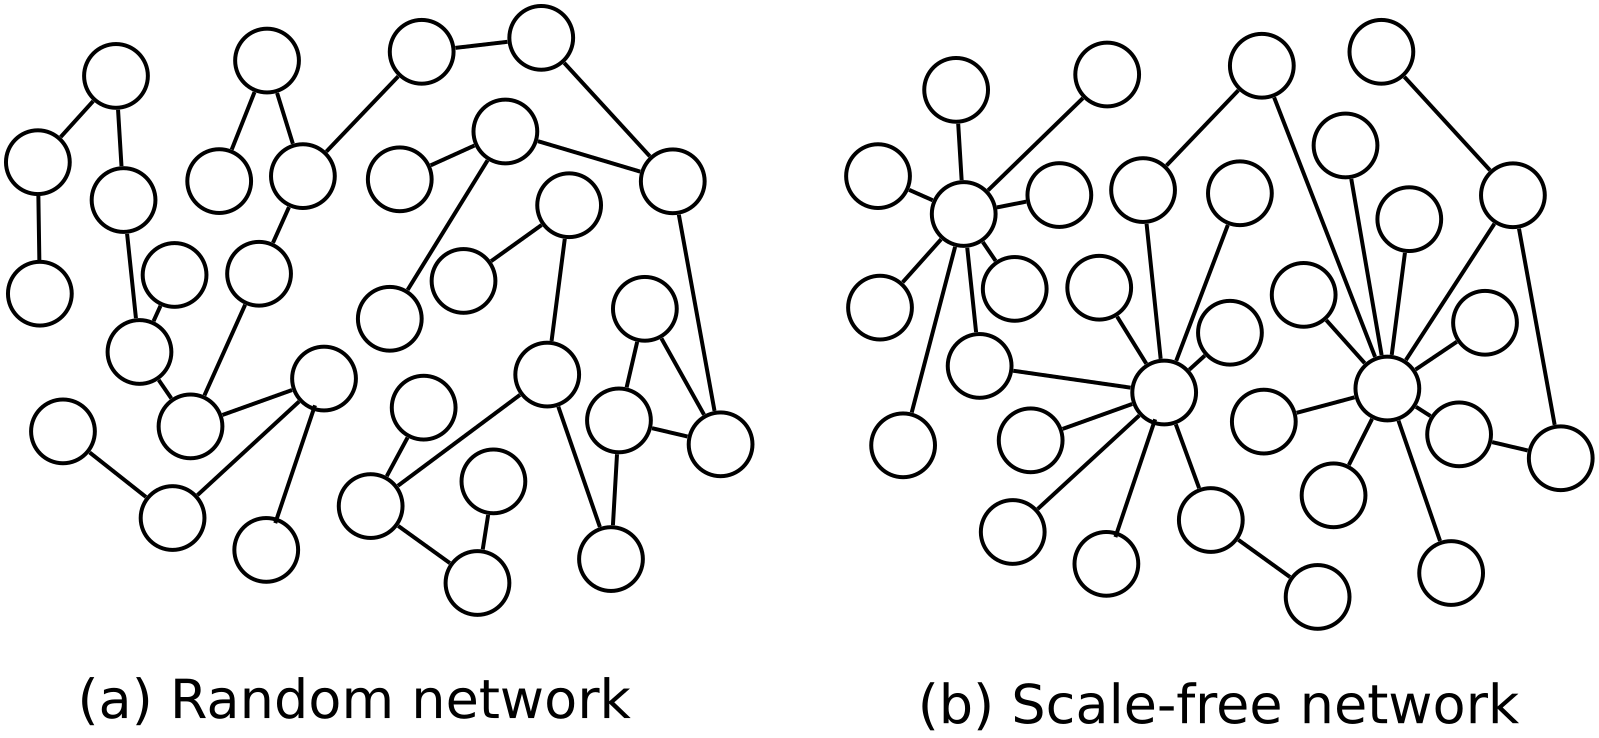
\includegraphics[width=0.4\textwidth]{scale_free_network.png}
  \end{figure}
  \begin{figure}
    \centering
    \textbf{Degree distribution}\par\medskip
    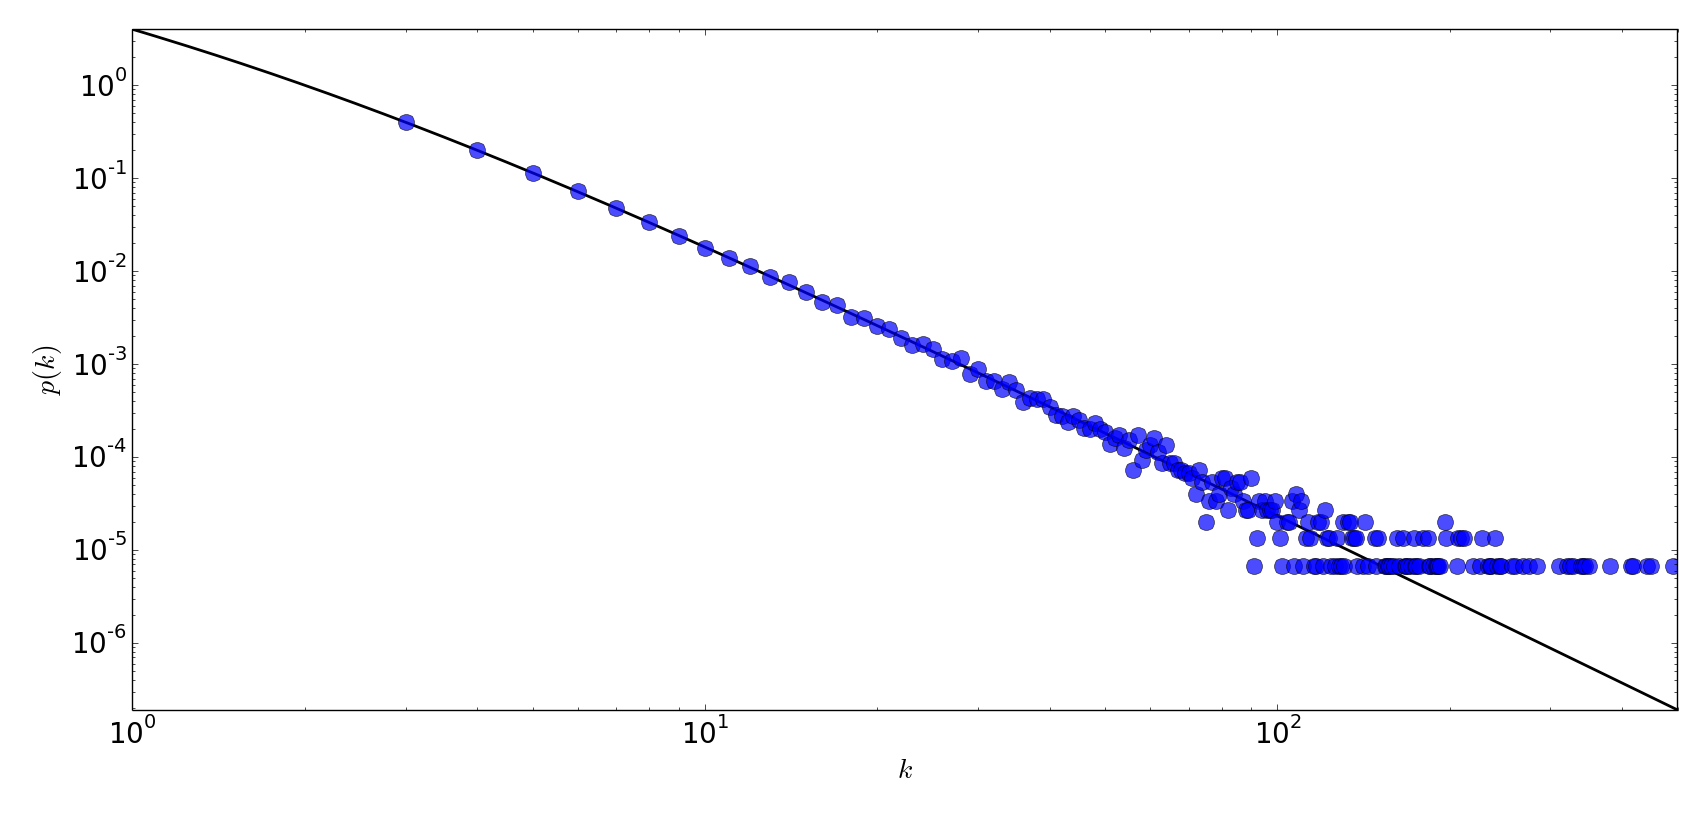
\includegraphics[width=0.4\textwidth]{scale_free_distribution.png}
    \caption{Degree distribution for a network with 150000 vertices and mean degree = 6 created using the Barabási–Albert model (blue dots). The distribution follows an analytical form given by the ratio of two gamma functions (black line) which approximates as a power-law.}
  \end{figure}
\end{frame}


\begin{frame}{References}
    \printbibliography
\end{frame}

\begin{frame}{}
  \centering \Huge
  \emph{Thanks for listening!}
\end{frame}

\end{document}



